\documentclass{beamer}
\usepackage[spanish]{babel}
\usepackage[utf8]{inputenc}
\usepackage{beamerthemeshadow}
\usepackage{pgf}

\usetheme{CambridgeUS}
\usefonttheme{structurebold}

\setbeamertemplate{itemize item}[triangle]


\begin{document}

\title{Realidad aumentada en Android}
\subtitle{Reconocimiento de imágenes y geolocalización usando Google Maps}
\author[Nacho Álvarez]
{
  \begin{tabular}[h]{cc}
      Nacho Álvarez\\
      @neonigmacdb
  \end{tabular} 
}

\institute[WUL4]{WUL4 (What You Look For)}
\date{\today}



\frame{\centering 
\includegraphics[height=1cm]{imgs/gdgdevfest.png} \titlepage}

\section[Índice]{}
\frame{\tableofcontents}

\section{Acerca de mí}
\frame
{
\frametitle{Who?}
\begin{itemize}
\item \textbf{Trayectoria:} soporte UCO, desarrollador Web, desarrollador / integrador distribuciones GNU/Linux.
\item \textbf{Actualmente:} WUL4 Córdoba (mobile + backend developer)
\item \textbf{Involucrado en:} \\ \vspace{10pt}
  $\vcenter{\hbox{
\includegraphics[height=1.25in]{imgs/wul4bus.jpg}}}$
  $\vcenter{\hbox{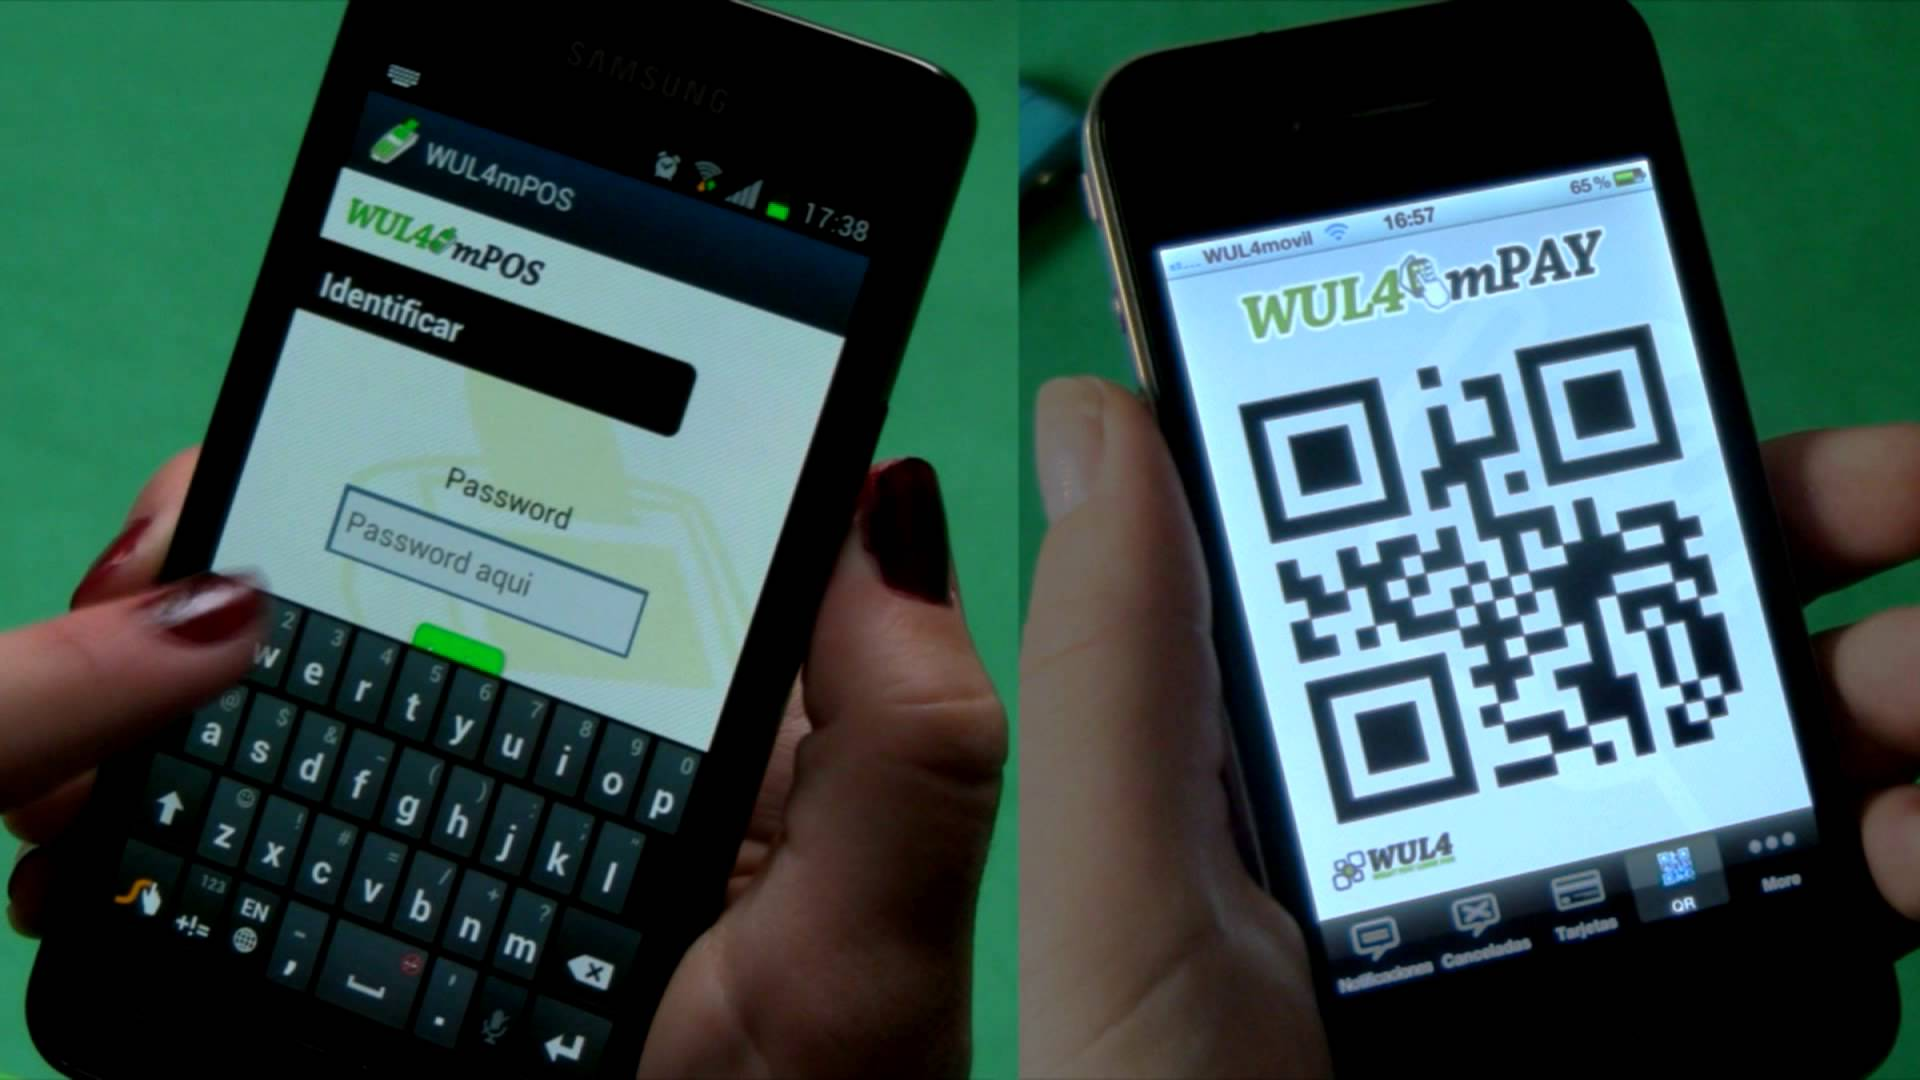
\includegraphics[height=1in]{imgs/wul4mpay.jpg}}}$
  $\vcenter{\hbox{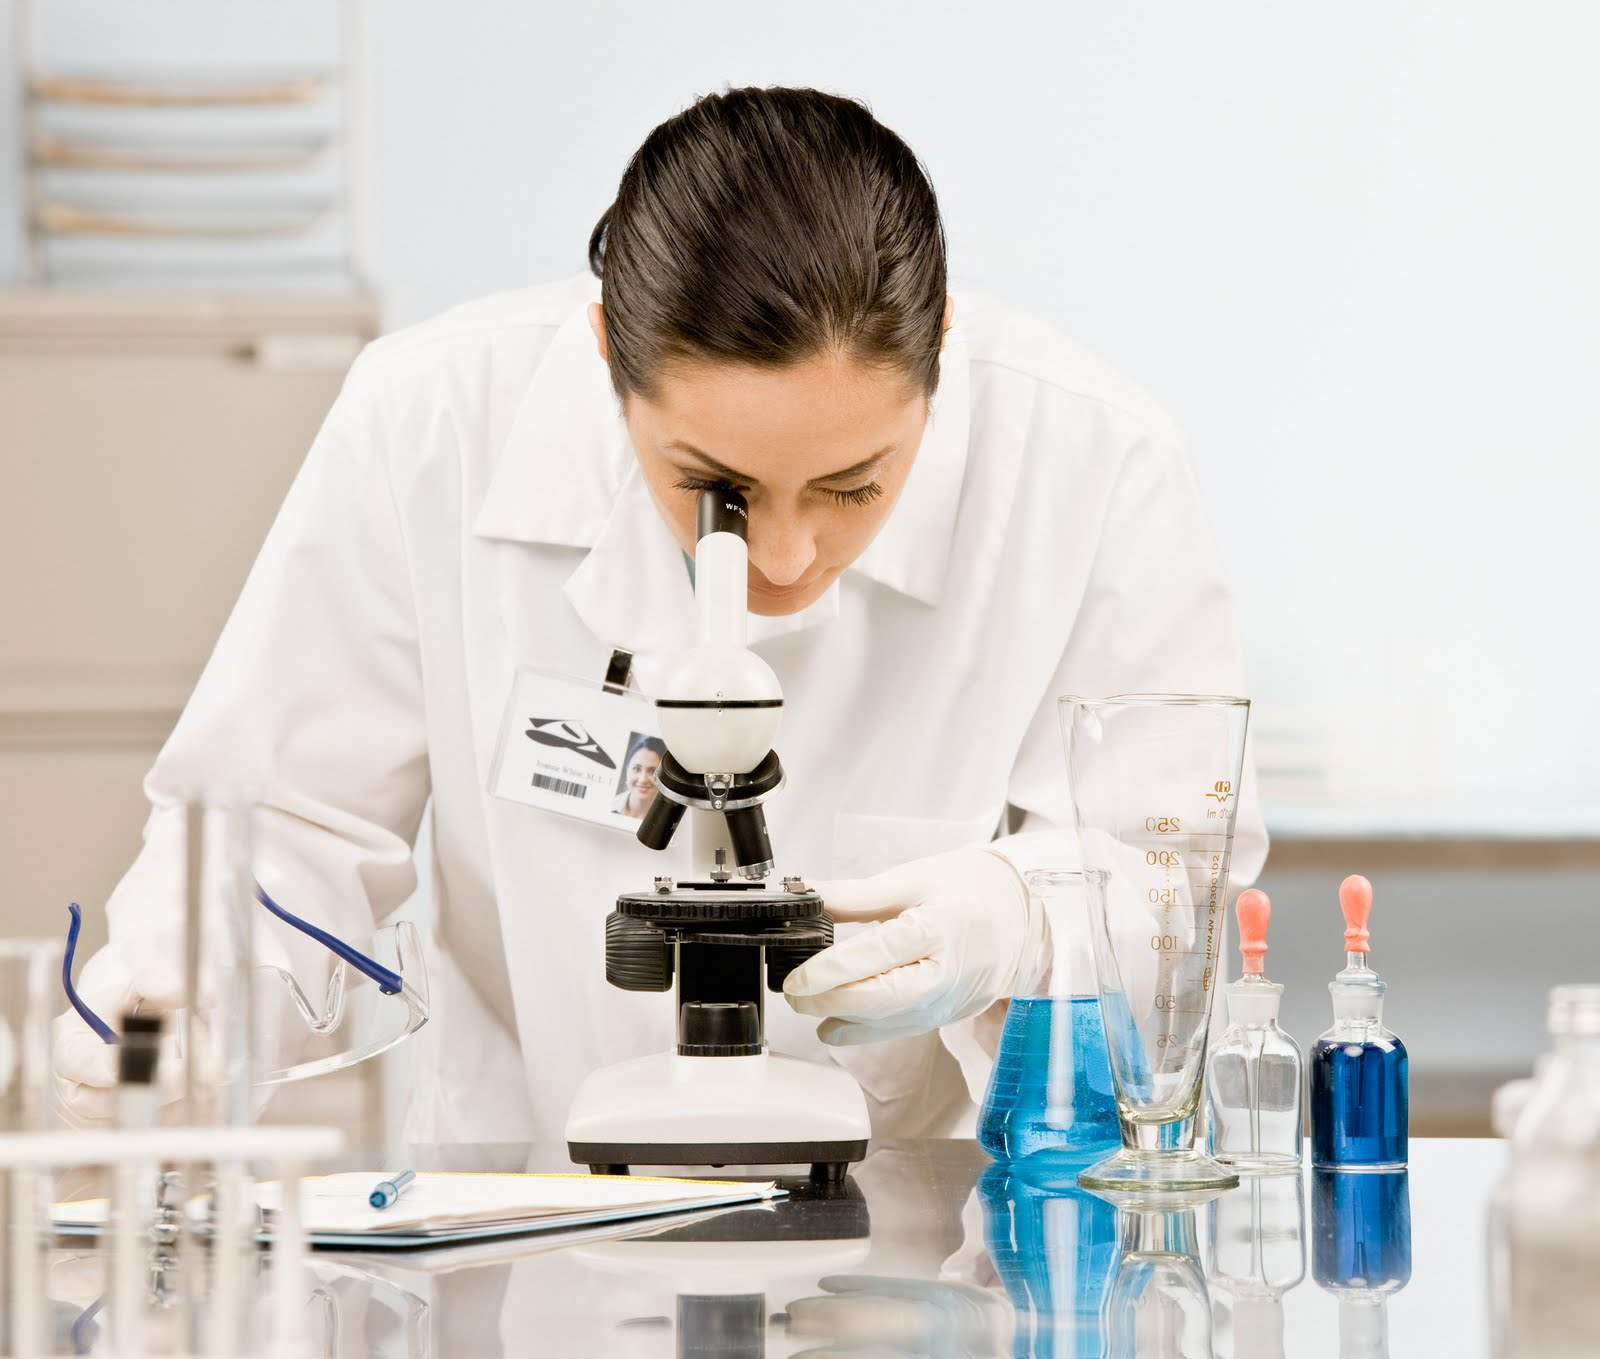
\includegraphics[height=1in]{imgs/id.jpg}}}$
\end{itemize}
}

%\section*{Sección 2}
\frame
{
\frametitle{}
\begin{center}
\begin{huge}
\hspace*{1cm}Conceptos asociados\newline\newline
\end{huge}
\includegraphics[width=0.5\textwidth]{imgs/conceptos.jpg}
\end{center}
}

\section{Conceptos asociados}
\frame
{
\frametitle{Introducción de conceptos}
\begin{itemize}
 \item Importante familiarizarse con algunos términos del mundillo.
 \item La razón es conocer de forma general qué papel juegan ciertos elementos en los procesadores.
 \item Una visión clara de los conceptos asociados al tema nos facilita la elección de un procesador.
\end{itemize}
}

\frame
{
\frametitle{Socket de CPU}
\begin{itemize}
 \item El \textbf{socket de CPU} es una matriz de pequeños agujeros (zócalo) existente en una placa base donde encajan los pines de un microprocesador; dicha matriz, denominada \textit{Pin grid array} o PGA, permite la conexión entre el microprocesador y dicha placa base.
 \item Ejemplos de socket de CPU son: Socket 939 (AMD), Socket AM2 (AMD), Socket 478 (Intel), Socket 775 (Intel)...\vspace*{0.5cm}

\hspace*{3cm}
\includegraphics[width=1.5cm]{imgs/socket939.jpg}
\hspace*{1cm}
\includegraphics[width=3.5cm]{imgs/socket775.jpg}

\end{itemize}
}

\frame
{
\frametitle{Niveles de caché}
\begin{itemize}
 \item \textbf{Propósito de la caché:} actuar como una memoria temporal entre los registros de CPU, limitados y de gran velocidad y la RAM, mucho más grande y lenta.
 \item Los subsistemas de caché pueden ser de \textbf{niveles múltiples}; es decir, puede haber más de un conjunto de caché entre el CPU y la memoria principal. 
 \item Muchos sistemas tienen \textbf{dos niveles de caché}:
	\begin{itemize}
	\item \underline{Caché L1}  $\Rightarrow$ ubicada en el chip de la CPU, se ejecuta a la misma velocidad que dicha CPU.
	\item \underline{Caché L2} $\Rightarrow$ suele ser parte del módulo de la CPU, se ejecuta a las mismas velocidades que la CPU (o casi) y es un poco más grande y lenta que la caché L1.
	\end{itemize}
 \item Algunos sistemas (normalmente servidores) también tienen \textbf{caché L3} formando parte del sistema de la placa base. La caché L3 es más grande y  algo más lenta que la caché L2.
\end{itemize}
}

\frame
{
\frametitle{MMX}
\begin{itemize}
 \item Es el acrónimo de \textbf{M}ulti\textbf{m}edia E\textbf{x}tensions.
 \item Conjunto de instrucciones \textbf{SIMD} (Single Instruction Multiple Data) diseñado por Intel e introducido en 1997 en sus microprocesadores Pentium MMX.
 \item MMX agregó \textbf{8 nuevos registros} a la arquitectura, conocida como MM0 a MM7. En realidad, estos nuevos registros son meros alias de los registros de la pila de la FPU. Cada uno de los registros MMn es un número entero de 64 bits.
 \item El juego de instrucciones MMX utiliza el concepto del \textbf{tipo de datos compactados} $\Rightarrow$ en lugar de usar el registro completo para un solo número entero de 64 bits, se usa para almacenar dos enteros de 32 bits, cuatro enteros de 16 bits u ocho enteros de 8 bits.
 \item \textbf{Problema:} MMX sólo soporta operaciones con números enteros. Hace algún tiempo, el uso de matemáticas de vector entero tenía sentido (operaciones 2D y 3D), pero cuando esta funcionalidad se pasa a las GPUs, la coma flotante se vuelve mucho más importante.
 \end{itemize}
}

\frame
{
\frametitle{SSE}
\begin{itemize}
 \item \textbf{SSE} (Streaming SIMD Extensions) es una extensión al grupo de instrucciones MMX.
 \item Estas instrucciones operan con paquetes de operandos en \textbf{coma flotante} de precisión simple.
 \item Hay varios tipos de instrucciones SSE:
	\begin{itemize}
		\item Instrucciones SSE de Transferencia de datos.
 		\item Instrucciones SSE de Conversión.
 		\item Instrucciones SSE Aritméticas.
 		\item Instrucciones SSE lógicas.
	\end{itemize}
 \item Con la tecnología SSE, se introducen 70 nuevas instrucciones y 8 registros nuevos: del xmm0 al xmm7.
 \item Los registros tienen una extensión de 128 bits. A diferencia de MMX, la utilización de SSE no implicaba la inhabilitación de la FPU, por lo que no era necesario habilitarla nuevamente, lo que significaba para MMX pérdida de velocidad.
\end{itemize}
}

\frame
{
\frametitle{FSB (Front Side Bus)}
\begin{itemize}
 \item La CPU está conectada a \textbf{un bus} que le permite comunicarse con el resto de dispositivos.
 \item Gracias a este bus frontal de datos, llamado \textbf{FSB} (Front Side Bus), la CPU recibe información y la envía a otros dispositivos.
 \item El FSB se encuentra conectado al chip \textbf{Northbridge}, que es el núcleo de la placa base.
 \item La frecuencia de un procesador se expresa en términos de la \textbf{frecuencia del FSB} multiplicado por un valor predeterminado por el fabricante, por eso conocer bien el FSB es vital en la práctica del Overclocking (forzar un procesador a trabajar a una velocidad mayor que la de serie).
 \item \textbf{Ejemplo} $\Rightarrow$ \textbf{Multiplicador:} x18, \textbf{Frecuencia del FSB:} 200MHz, \textbf{Frecuencia del procesador:} 3600 MHz.
\end{itemize}
}

\frame
{
\frametitle{FSB (Front Side Bus)}
\begin{center}
\includegraphics[width=0.6\textwidth]{imgs/nsbridge.png}
\end{center}
}

%\section*{Sección 3}
\frame
{
\frametitle{}
\begin{center}
\begin{huge}
\hspace*{1cm}Un baile de tecnologías\newline\newline
\end{huge}
\includegraphics[width=0.4\textwidth]{imgs/tecnologias.jpg}
\end{center}
}

\section{Un baile de tecnologías}
\frame
{
\frametitle{Tecnologías empleadas por los principales competidores}

\begin{itemize}
 \item \textbf{Tecnologías empleadas por INTEL:}

	\begin{itemize}
	 \item Hyper-Threading
	 \item Intel 64 Architecture
	 \item Bit de desactivación de ejecución y seguridad
	\end{itemize}

\item \textbf{Tecnologías empleadas por AMD:}

	\begin{itemize}
	 \item HyperTransport
	 \item AMD 64
	 \item Bit NX
	\end{itemize}

\end{itemize}
}

\frame
{
\frametitle{Tecnologías empleadas por INTEL}
\begin{itemize}
 \item \textbf{Hyper-Threading:}
 \begin{itemize}
  \item Dos formas de brindar más potencia informática:
	\begin{enumerate}
	 \item Aumentar la velocidad del reloj.
	 \item Realizar más trabajo en \textbf{cada ciclo de reloj}.
	\end{enumerate}
  \item Un procesador \textit{compatible} con la tecnología Hyper-Threading se presenta a sí mismo ante las aplicaciones y los S.O. como dos \textbf{procesadores virtuales}.
  \item El procesador puede entonces trabajar en \textbf{dos conjuntos de tareas} a la vez, utilizar los recursos que de otro modo estarían inactivos y realizar más trabajo en la misma cantidad de tiempo.
  \item En los \textbf{PC de escritorio:}
	\begin{itemize}
	 \item La tecnología HT aprovecha la capacidad de subprocesos múltiples integrada en WinXP y en muchas aplicaciones. El software con subprocesos múltiples divide su carga de trabajo en procesos y subprocesos que se pueden programar y enviar de forma independiente. Es parecido a un sistema multiprocesador pero con \underline{un único procesador}.
	\end{itemize}
 \end{itemize}
\end{itemize}
}

\frame
{
\frametitle{Tecnologías empleadas por INTEL}
\begin{itemize}
  \item En los \textbf{servidores:}
	\begin{itemize}
	 \item La tecnología HT permite el paralelismo a nivel de subprocesos al duplicar el estado arquitectónico de cada procesador a la vez que se comparte un conjunto de recursos de ejecución del procesador. Cuando programa subprocesos, el SO considera los dos estados arquitectónicos claramente determinados como procesadores ``lógicos'' separados
	\end{itemize}
 
\begin{center}
  \includegraphics[width=0.6\textwidth]{imgs/ht.png}
\end{center}
\end{itemize}
}

\frame
{
\frametitle{Tecnologías empleadas por INTEL}
\begin{itemize}
 \item \textbf{Intel 64:}

	\begin{itemize}
		\item La arquitectura \textbf{Intel 64} proporciona \textbf{computación de 64 bits} cuando se combina con \underline{software que la soporte}. 
		\item Mejora el rendimiento permitiendo a los sistemas direccionar\textbf{ más de 4 gigabytes} tanto de \textbf{memoria virtual} como \textbf{física}.
 	\end{itemize}

 \item \textbf{Bit de desactivación de ejecución y seguridad:}

	\begin{itemize}
		\item Previene ciertos tipos de ataques de \textbf{desbordamiento de buffer} cuando se combina con un sistema operativo compatible.
		\item Permite que el procesador clasifique \textbf{áreas de la memoria} en función de dónde se puede ejecutar el código de las aplicaciones.\newline
	\end{itemize}

\begin{center}
\scriptsize \fbox{
\begin{minipage}{11cm}
Si un gusano intenta \textbf{insertar código en el buffer}, el procesador desactiva la ejecución del código, lo cual evita el daño y la propagación del gusano.
\end{minipage}
}
\end{center}
\end{itemize}
}

\frame
{
\frametitle{Tecnologías empleadas por AMD}
\begin{itemize}
 \item \textbf{HyperTransport:}

	\begin{itemize}
		\item Tecnología que induce en una \textbf{mejora de las prestaciones} del sistema, diseñada para incrementar las mismas mediante la \textbf{eliminación de cuellos de botella en la E/S}, lo cual mejora notablemente el ancho de banda y reduce la \textit{latencia}. 

		\item Las mejoras se centran en cuatro apartados:

		\begin{itemize}
		 \item[1)] \textbf{FSB del procesador:} Sustituyendo el FSB por unas conexiones de E/S basadas en la tecnología HyperTransport se consigue una \textbf{extensión del ancho de banda} desde los 2,1GB/s hasta los 6,4GB/s.

		 \item[2)] \textbf{Interfaz de memoria:} Cuando ocurre un fallo en la caché, el procesador debe traer información de memoria principal. En Northbridge/Southbridge, las transacciones de memoria pasan por el chip Northbridge, creando latencias adicionales. Para resolver este cuello de botella, AMD incorpora el controlador de memoria en su 8ª generación de procesadores. 

		\end{itemize}
	\end{itemize}
\end{itemize}
}

\frame
{
\frametitle{Tecnologías empleadas por AMD}
\begin{itemize}
 \item \textbf{HyperTransport:}

	\begin{itemize}
		\item Las mejoras se centran en cuatro apartados:

		\begin{itemize}
		 \item[3)] \textbf{Interconexión chip a chip:} La \textbf{integración simultánea} de las tecnologías de alta velocidad como AGP-8x, Gigabit Ethernet, PCI-X, etc. elimina virtualmente los cuellos de botella en la E/S.

		 \item[4)] \textbf{Capacidades de expansión de E/S hacia la industria de buses de alta velocidad:} La arquitectura Northbridge/Southbridge no está preparada para soportar más de dos \textit{núcleos lógicos}, ya que la funcionalidad debería fijarse a una interfaz existente, y un bus actual no tendría suficiente ancho de banda para soportar tecnologías de alta velocidad.
		\end{itemize}
	\end{itemize}
\end{itemize}
}

\frame
{
\frametitle{Tecnologías empleadas por AMD}
\begin{itemize}
 \item \textbf{HyperTransport:}

	\begin{center}
	\includegraphics[width=0.8\textwidth]{imgs/htransport.png}
	\end{center}

\end{itemize}
}

\frame
{
\frametitle{Tecnologías empleadas por AMD}
\begin{itemize}
 \item \textbf{AMD64:} es una arquitectura basada en la \textbf{extensión} del conjunto de instrucciones x86 para manejar direcciones de 64 bits. Además, contempla mejoras adicionales como \textbf{duplicar el número y el tamaño} de los registros de uso general y de instrucciones SSE.

 \item \textbf{Bit NX:} el bit NX es una característica del procesador que permite al SO prohibir la ejecución del código en ciertas áreas de datos. 
\end{itemize}
}

%\section*{Sección 4}
\frame
{
\frametitle{}
\begin{center}
\begin{huge}1 núcleo, 2 núcleos, 4 núcleos... Un poco \hspace*{1.5cm}de historia.\newline\newline
\end{huge}
\includegraphics[width=0.25\textwidth]{imgs/amd-opteron.jpg}\hspace*{1cm}
\includegraphics[width=0.28\textwidth]{imgs/intel-quad.jpg}
\end{center}
}

\section{1 núcleo, 2 núcleos, 4 núcleos... Un poco de historia.}
\frame
{
\frametitle{¿Necesitamos tanta capacidad?}
\begin{itemize}
\item La enferma carrera que mantienen Intel y AMD por superar al rival nos lleva a ver morir productos que ni siquiera pudimos consumir ni necesitábamos hacerlo.
\item Muchos ni siquiera disponemos aún de un procesador de doble núcleo, ni en el PC de escritorio ni en el portátil.
\item Es posible saltarse hasta una generación de procesadores en la compra de nuestro próximo equipo.
\end{itemize}
}

\frame
{
\frametitle{AMD vs. Intel y una carrera que no para}
\begin{itemize}
\item AMD lanzó sus procesadores doble núcleo, los Athlon64 X2, luego Intel hizo lo propio con su línea Pentium D.
\item Pentium D utilizaba la tecnología NetBurst, con cuello de botella para los datos y no alcanzaba en rendimiento a Athlon 64 X2.
\item Intel contraataca con los Core Duo, con nueva tecnología y diseño de 65 nanómetros. Más tarde, actualiza la tecnología a la actual \textbf{Core 2 Duo}.
\end{itemize}
}

\frame
{
\frametitle{Pero, ¿qué es doble núcleo?}
\begin{itemize}
\item Esta pregunta tan manida significa que la CPU, tiene no un procesador, si no dos en el mismo paquete y se distribuyen el trabajo.
\item Lo lógico es pensar que al tener dos cerebros se puede procesar el doble de información, pero, lamentablemente, no siempre es así.
\item Dos factores justifican esta limitación:

	\begin{itemize}
	\item[1)] \textbf{Ancho de banda / cuello de botella}
		\begin{itemize}
		\item Problema común en los Pentium D, que \textbf{comparten el FSB} para recibir información y devolverla procesada.
		\item El FSB está \textbf{limitado en ancho} y encima es compartido por ambos núcleos, por lo que los datos deben esperar su turno para procesarse.
		\item \textbf{AMD} creó la interconexión \textbf{HyperTransport}, que interconecta los núcleos en varias direcciones, lo que proporciona un canal directo entre el procesador y la memoria sin tener que compartirlo con nadie. 
		\item Problema de AMD $\Rightarrow$ cuando AMD estaba utilizando un \textbf{método de fabricación} de 130nm, Intel pasó al de 90nm, cuando AMD al fin pudo llegar a 90nm Intel se volvió a adelantar con el de 65nm.
		\item La ventaja de poder incluir \textbf{más en menos espacio} y que las conexiones y distancias de los circuitos sean más pequeñas es que se necesita menos energía para mover un electrón de un lugar al otro.
		\end{itemize}
	\end{itemize}
\end{itemize}
}

\frame
{
\frametitle{Pero, ¿qué es doble núcleo?}
\begin{itemize}
 	\item Dos factores justifican esta limitación:

	\begin{itemize}
	\item[2)] \textbf{Aplicaciones}

		\begin{itemize}
		\item \textbf{Pocas aplicaciones preparadas} para sacar provecho de dos núcleos (incluidos los juegos).
		\item El único lugar donde se saca realmente provecho es del \textbf{lado servidor} y procesamiento de video.
		\item Gran ventaja con múltiples núcleos $\Rightarrow$ renderizando una \textbf{imagen 3D de alta resolución}, cada núcleo se puede encargar de un frame, tener muchos núcleos nos multiplicaría el tiempo ahorrado.
		\item Por esta razón se utilizan \textbf{granjas de servidores} para procesar películas.
		\item Básicamente se aprovechan las ventajas en todas las tareas que se puedan dividir en hilos y no ser todo un conjunto de procesamiento.
		\end{itemize}

	\end{itemize}

\end{itemize}
}

\frame
{
\frametitle{Quad core: 4 núcleos efectivos.}
\begin{itemize}
\item \textbf{AMD: pionera} con su AMD Quad FX (AMD 4x4 antes de su lanzamiento).
\item Emplea \textbf{dos zócalos AM2} con HyperTransport, cada uno de los cuales permite una \textbf{CPU de doble núcleo} y un banco de \textbf{memoria DDR2}.
\item \textbf{Intel} contraataca con dos Core 2 Duo en un mismo paquete compartiendo el bus de datos a la memoria, llamándolos:
	\begin{itemize}
	\item \textbf{Core 2 Quad:} procesadores con 4 núcleos y de 64 bits. Son un 70\% más rápidos que los Core 2 Duo.
	\item \textbf{Core 2 Extreme:} tienen multiplicador desbloqueado (hasta 40x), y se utilizan los mejores cristales en su fabricación, con lo cual el proceso de overclocking es más sencillo y tiene un potencial más alto.
	\end{itemize}
\item \textbf{Para portátiles:} en el primer semestre de 2008 se actualizan los denominados \textbf{Intel Santa Rosa} con la tecnología \textbf{Core 2 Quad}. Los procesadores serán los llamados \textbf{\textit{Penryn}}.
\end{itemize}
}

\frame
{
\frametitle{Quad core: 4 núcleos efectivos.}
\begin{itemize}
 \item La ``competición'' no termina aquí: mientras Intel vende microprocesadores de cuatro núcleos que son \textbf{dos paquetes de dos núcleos cada uno}, AMD lanza los Opteron (nombre clave \textbf{\textit{Barcelona}}), con cuatro núcleos de verdad individuales dentro del propio procesador.
 \item El mercado de servidores se encuentra ahora con la dualidad AMD Opteron - Intel Xeon (Core 2 Extreme), ambos con 4 núcleos.
 \item Por si fuera poco, AMD lanza \textbf{\textit{Phenom}} para equipos de sobremesa, que llegan al mercado en el primer trimestre de 2008. Las versiones de triple núcleo (nombre código ``Toliman'') formarán las series \textit{Phenom 8000}, las versiones de cuatro núcleos (nombre código ``Agena'') formarán las series \textit{Phenom 9000}, y las versiones de gama alta (nombre código ``Agena FX'') serán las series \textit{Phenom FX}.
 \item No consiguen derrotar a \textbf{\textit{Intel Core 2 Quad}} ni siquiera en la que se suponía su mayor baza (consumo energético) ni en escala de integración (Intel utiliza ya ¡45nm!).

\end{itemize}
}

\frame
{
\frametitle{Curiosidades...}
\begin{itemize}
 \item Para identificar la información de un procesador:
\end{itemize}

\begin{center}
 \includegraphics[width=0.8\textwidth]{imgs/howto-procesador.png}
\end{center}
}

\frame
{
\frametitle{Curiosidades...}
\textbf{Shrek Tercero} se diseñó con el siguiente hardware:
\hspace*{2cm} \includegraphics[width=1cm]{imgs/shrek3.jpg}
\begin{itemize}
\item Servidores \textbf{HP ProLiant DL145} compuestos por procesadores \textbf{AMD Opteron} de doble núcleo y \textbf{8GB de RAM.}
\item Estaciones de trabajo \textbf{HP xw9300} compuestas de igual manera por procesadores \textbf{AMD Opteron} de doble núcleo.
\item Portátiles \textbf{HP nx6125} basadas en el procesador \textbf{AMD Turion64 X2}.
\item Para elaboración de la película se utilizaron la cantidad de 4000 núcleos es decir 2000 procesadores.
\item En 2001, \textbf{Shrek I} necesitó 5 millones de horas de CPU. En 2004, \textbf{Shrek 2 } precisó 10 millones, y en 2007 \textbf{Shrek 3} preciśo 20 millones.
\item El almacenamiento de Shrek 3 precisa 24 TB.
\end{itemize}
	\scriptsize \fbox{
	\begin{minipage}{11cm}
	Linux Red Hat Enterprise 4 como SO y Python para escribir las utilidades software.
	\end{minipage}
	}
}

%\section*{Sección 5}
\frame
{
\frametitle{}
\begin{center}
\begin{huge}
\hspace*{1cm}¿Y qué hay de los portátiles?\newline
\end{huge}
\includegraphics[width=0.8\textwidth]{imgs/portatiles.png}
\end{center}
}

\section{¿Y qué hay de los portátiles?}
\frame
{
\frametitle{Los procesadores móviles de Intel}
\begin{itemize}
 \item Ni mucho menos el avance en el diseño de \textbf{procesadores para portátiles} se ha quedado estancado.
 \item Intel ofrece las tecnologías \textbf{Centrino} y \textbf{Centrino Duo}.
 \item Son \textbf{tecnologías} desarrolladas para promocionar en el diseño de un ordenador portátil una combinación determinada de:

	\begin{itemize}
	\item CPU Intel Pentium M o, posteriormente, \textbf{Intel Core} o \textbf{Intel Core 2}.
	\item Chipset de la placa base familia Intel \textbf{855}, \textbf{915} o \textbf{945}.
	\item Interface de red inalámbrica del tipo Intel PRO/Wireless \textbf{2100 (IEEE 802.11a/b)} o PRO/Wireless 2200 \textbf{(IEEE 802.11b/g)} o posterior.
	\end{itemize}

 \item No se debe confundir al procesador Pentium M como ``el procesador Centrino'', ya que Centrino es \textbf{la tecnología} que engloba al procesador, al chipset y a la tarjeta de red inalámbrica Wi-Fi integrada.

\end{itemize}
}

\frame
{
\frametitle{Los procesadores móviles de Intel}
\begin{itemize}
 \item Intel diseñó su estrategia en base a una serie de \textbf{plataformas}:
	\begin{itemize}
		\item \textbf{\underline{Plataforma Carmel}}\\
		Plataforma original Centrino, lanzada en 2003. Consta de:
		\begin{itemize}
		\item CPU Pentium-M (nombre clave \textit{Banias}) bus 400 MHz, 1MB Caché L2.
		\item Chipset serie 855.
		\item Chip WiFi Intel PRO/Wireless 2100 o 2200.
		\end{itemize}
	
		\item \textbf{\underline{Plataforma Sonoma}}\\
		Plataforma que actualiza la original con la nueva generación de Centrino, lanzada en 2005. Consta de:
		\begin{itemize}
		\item CPU Pentium-M (algunos incluyen el núcleo mejorado con nombre clave \textit{Dohan}) bus 533 MHz, 2MB Caché L2.
		\item Chipset serie 915.
		\item Tecnología PCI Express.
		\item Chip WiFi Intel PRO/Wireless 2915 (IEEE 802.11a/b/g).
		\end{itemize}	
	\end{itemize}
\end{itemize}
}

\frame
{
\frametitle{Los procesadores móviles de Intel}
\begin{itemize}
 \item Intel diseñó su estrategia en base a una serie de \textbf{plataformas}:
	\begin{itemize}
	 \item \textbf{\underline{Plataforma Napa}}\\
	Versión de Centrino lanzada en 2006. Consta de:
		\begin{itemize}
		\item CPU Core Solo (Duo mononúcleo), Core Duo (nombre clave \textit{Yonah}) o posteriormente Core 2 Duo (\textit{Merom}). Las versiones de la plataforma Centrino basadas en CPU \textbf{Core Duo} y \textbf{Core 2 Duo} reciben el nombre de \textbf{Centrino Duo}.
		\item Chipset serie 945, que puede incluir gráficos integrados GMA950.
		\item Intel PRO/Wireless 3945 IEEE 802.11 a/b/g.
		\end{itemize}
	\end{itemize}

	\begin{itemize}
	 \item \textbf{\underline{Plataforma Santa Rosa} * Plataforma vigente en la actualidad *}\\
	Es la cuarta generación de la plataforma Centrino. Presentado el 9 de mayo de 2007, con:
		\begin{itemize}
		\item CPU Core 2 Duo (Merom 2ª generación).
		\item Chipset serie 965 (con gráficas integradas X3000, nombre clave \textit{Crestiline}).
		\item Intel PRO/Wireless 4965AGN IEEE 802.11 a/b/g/n.
		\end{itemize}
	\end{itemize}
\end{itemize}
}

\frame
{
\frametitle{Los procesadores móviles de Intel}
\begin{itemize}
 \item Intel diseñó su estrategia en base a una serie de \textbf{plataformas}:
	\begin{itemize}
	 \item \textbf{\underline{Plataforma Santa Rosa} * Plataforma vigente en la actualidad *}\\
	Analizando algo más en detalle:
		\begin{itemize}
		\item Se comercializan con los nombres de \textbf{Centrino Duo} (como los anteriores) y \textbf{Centrino Pro}.
		\item Se incluyen nuevos modelos de procesadores de 65 nm: los Core 2 T7x00, con 4 MB de caché L2 y FSB a 800 MHz.
		\item Incorporan la tecnología \textbf{Turbo Memory}, que sirve para emplear una memoria flash a modo de caché del disco duro para \textbf{aumentar el rendimiento} y \textbf{reducir el consumo}.
		\item Opinión personal: realmente rápido utilizando \textbf{Ubuntu}, compilando, instalando paquetes, etc...
		\end{itemize}
	\end{itemize}
\end{itemize}
}

\frame
{
\frametitle{Los procesadores móviles de Intel}
\begin{itemize}
 \item Intel diseñó su estrategia en base a una serie de \textbf{plataformas}:
	\begin{itemize}
	 \item \textbf{\underline{Plataforma Montevina}}\\
	El nombre código \textit{Montevina} se refiere a la quinta generación de la plataforma Centrino. Esta prevista para lanzarse a inicios del 2008. Montevina soportará:

		\begin{itemize}
		\item Procesador de ¡45nm! \textbf{Penryn} (4 núcleos).
		\item Chipset \textbf{Cantiga}, con FSB a \textbf{1GHz}.
		\item El módulo inalámbrico \textbf{Shiloh}, con soporte para \textbf{WiMAX} y \textbf{HSDPA} (optimización de UTMS, se le reconoce como 3.5G), además del controlador \textbf{LAN Boaz}.
		\item Memorias DDR3 (por confirmar).
		\end{itemize}
	\end{itemize}
\end{itemize}
}

\frame
{
\frametitle{Los procesadores móviles de AMD}
\begin{itemize}
 \item AMD basa su estrategia comercial para portátiles en \textbf{tres familias de procesadores}:

	\begin{itemize}
		\item \textbf{\underline{Mobile AMD Sempron}}\\
		Microprocesador de bajo coste con arquitectura X86 que se equipara al procesador Celeron de Intel. Las primeras versiones fueron lanzadas al mercado en agosto de 2004.
		\item \textbf{\underline{AMD \underline{Athlon} 64 X2 Dual-Core}}
		\begin{itemize}
			\item Microprocesador de 64 bits y doble núcleo. Consta de:
			\item Versiones para el Socket 939 (en 90 nm) y para el socket AM2 (en 90 nm y 65 nm).
			\item Bus HyperTransport de 2000 Mhz.
			\item Soporte de memoria DDR2 a partir de los modelos AM2 (Julio 2006) y conjunto de instrucciones SSE3.
		\end{itemize}
	\end{itemize}
\end{itemize}
}

\frame
{
\frametitle{Los procesadores móviles de AMD}
\begin{itemize}
 \item AMD basa su estrategia comercial para portátiles en \textbf{tres familias de procesadores}:

	\begin{itemize}
		\item \textbf{\underline{AMD \underline{Turion} 64 X2 Dual-Core}}\\
		Versión de bajo consumo del procesador AMD Athlon 64 destinada a portátiles. Constituye la respuesta comercial de AMD a la plataforma Centrino de Intel. Los modelos disponibles son:\vspace*{0.3cm}

		\item Lancaster (90 nm)
			\begin{itemize}
			\item Caché L2: 512 o 1024 KB.
			\item Socket 754, HyperTransport (800 MHz, HT800).
			\item Lanzamiento: 10 de marzo, 2005.
			\item Frecuencias de reloj: hasta 2400 MHz.
			\end{itemize}

		\item Richmond (65nm y 90nm)
			\begin{itemize}
			\item Como los Lancaster, salvo que se añade tecnología de virtualización AMD-V.
			\end{itemize}
	\end{itemize}
\end{itemize}
}


%\section*{Sección 6}
\frame
{
\frametitle{}
\begin{center}
\begin{huge}Comparando los distintos procesadores\newline\newline
\end{huge}
\includegraphics[width=0.3\textwidth]{imgs/comparison1.png}\hspace*{1cm}
\includegraphics[width=0.3\textwidth]{imgs/comparison2.jpg}
\end{center}
}

\section{Comparando los distintos procesadores}
\frame
{
\frametitle{Cómo vamos a realizar la comparación}
\begin{itemize}
 \item Vamos a analizar las especificaciones de los procesadores de las compañías líderes mediante unas tablas de datos.
 \item Nos centramos en el hecho de que un procesador teóricamente idéntico que otro con el mismo nombre clave es inferior debido a que difieren en el número de procesador.
 \item Cada número de procesador nos marca unas características.
 \item Cada compañía tiene un \textit{sitio Web} con utilidades de comparación de sus procesadores.
	\begin{itemize}
	\item \textbf{Intel} $\Rightarrow$ http://compare.intel.com
	\item \textbf{AMD} $\Rightarrow$ http://www.amdcompare.com
	\end{itemize}
 \item Diferenciamos entre equipos de sobremesa (escritorio) y equipos portátiles. Además, dividimos por compañía.
\end{itemize}
}

\frame
{
\frametitle{Procesadores Intel de escritorio}
\begin{itemize}
\item Consideraremos los siguientes procesadores Intel de escritorio:
	\begin{itemize}
	\item \textbf{Pentium D:} dos procesadores Pentium 4 (de núcleo \textit{Prescott}) \textbf{sin} HyperThreading con pequeñas mejoras internas, metidos ambos en una única pieza de silicio.
	\item \textbf{Pentium Extreme Edition:} no confundir con el Pentium 4 Extreme Edition, el Pentium \textbf{Extreme Edition} contiene dos procesadores \textit{Pentium 4 Prescott}, \textbf{con} tecnología Hyperthreading.
	\item \textbf{Pentium Dual Core:} basados en el procesador mononúcleo \textit{Conroe-L}, que no era suficiente para distinguir entre las marcas \textit{Pentium} y \textit{Celeron}, por lo que se sustituyó por CPUs de doble núcleo.
	\item \textbf{Intel Core 2 Duo:} la continuación de los \textit{Pentium D} y \textit{Core Duo} (éste último lanzado en enero de 2006). Nombre clave: \textit{Conroe}.
	\item \textbf{Intel Core 2 Quad:} procesadores con 4 núcleos y de 64 bits, un 70\% más rápidos que los \textit{Core 2 Duo}.
	\item \textbf{Intel Core 2 Extreme:} tienen multiplicador desbloqueado (hasta 40x), y se utilizan los mejores cristales en su fabricación, con lo cual el proceso de overclocking es más sencillo y tiene un potencial más alto.
	\end{itemize}
\end{itemize}
}

\frame
{
\frametitle{Procesadores Intel de escritorio}
\begin{itemize}
 \item \textbf{Tabla de especificaciones: procesador \textbf{Pentium D}}
\begin{center}
\includegraphics[width=0.9\textwidth]{imgs/tabla-pentium-d.png}
\end{center}
\end{itemize}
}

\frame
{
\frametitle{Procesadores Intel de escritorio}
\begin{itemize}
 \item \textbf{Tabla de especificaciones: procesadores \textbf{Pentium Dual Core y Extreme Edition}}
\begin{center}
\includegraphics[width=0.9\textwidth]{imgs/tabla-pentium-dual-y-extreme.png}
\end{center}
\end{itemize}
}

\frame
{
\frametitle{Procesadores Intel de escritorio}
\begin{itemize}
 \item \textbf{Tabla de especificaciones: procesador \textbf{Core 2 Duo}}
\begin{center}
\includegraphics[width=0.9\textwidth]{imgs/tabla-core2-duo.png}
\end{center}
\end{itemize}
}

\frame
{
\frametitle{Procesadores Intel de escritorio}
\begin{itemize}
 \item \textbf{Tabla de especificaciones: procesadores \textbf{Core 2 Quad y Core 2 Extreme}}
\begin{center}
\includegraphics[width=0.9\textwidth]{imgs/tabla-core2-quad-y-extreme.png}
\end{center}
\end{itemize}
}


\frame
{
\frametitle{Procesadores AMD de escritorio}
\begin{itemize}
\item Consideraremos los siguientes procesadores AMD de escritorio:
	\begin{itemize}
 	\item \textbf{AMD Athlon 64 X2 Dual Core:} microprocesador de 64 bits de doble núcleo introducido para el socket 939 (en 90 nm) y para el socket AM2 (en 90 nm y 65 nm) con un bus HyperTransport de 2000 Mhz y soporte de memoria DDR2 a partir de los modelos AM2, y conjunto de instrucciones SSE3. Cada núcleo cuenta con una unidad de cache independiente.
	\end{itemize}

\item Se han desestimado para el estudio los siguientes procesadores:
	\begin{itemize}
	 \item \textbf{AMD Sempron:} procesador mononúcleo.
	 \item \textbf{AMD Athlon 64:} procesador mononúcleo.
	 \item \textbf{AMD Athlon 64 FX:} procesador mononúcleo destinado principalmente al disfrute de juegos y multimedia.
	 \item \textbf{AMD Athlon X2 Dual Core:} son sólo tres modelos que salieron bajo dicho sobrenombre y que fueron un impulso cualitativo para los reales AMD Athlon 64 X2 Dual Core.
	\end{itemize}
\end{itemize}
}

\frame
{
\frametitle{Procesadores AMD de escritorio}
\begin{itemize}
 \item \textbf{Tabla de especificaciones: procesador \textbf{AMD Athlon 64 X2 Dual Core}}
\begin{center}
\includegraphics[width=0.9\textwidth]{imgs/tabla-amd-athlon64x2.png}
\end{center}
\end{itemize}
}

\frame
{
\frametitle{Procesadores Intel para portátiles}
\begin{itemize}
 \item Por la cantidad de procesadores existentes, aquí vamos a comparar las tecnologías \textit{Centrino}, \textit{Centrino Duo} y \textit{Centrino Pro}.
 \item \textbf{Tabla de especificaciones: procesadores \textbf{Core Solo (1 núcleo), Core 2 Solo (1 núcleo), Core Duo y Core 2 Duo}}:
\begin{center}
\includegraphics[width=0.8\textwidth]{imgs/tabla-centrinos.png}
\end{center}
\end{itemize}
}

\frame
{
\frametitle{Procesadores AMD para portátiles}
\begin{itemize}
\item Consideraremos los siguientes procesadores AMD para portátiles:
	\begin{itemize}
	\item AMD Athlon 64 X2 Dual-Core.
	\item AMD Turion 64 X2 Dual-Core.
	\end{itemize}

 \item \textbf{Tabla de especificaciones: procesadores AMD Athlon 64 X2 Dual Core y AMD Turion 64 X2 Dual-Core}
\end{itemize}

\begin{center}
\includegraphics[width=0.8\textwidth]{imgs/tabla-amd-turion-athlon.png}
\end{center}
}

%\section*{Sección 7}
\frame
{
\frametitle{}
\begin{center}
\begin{huge}Algunos datos de rendimiento\newline\newline
\end{huge}
\includegraphics[width=0.4\textwidth]{imgs/performance.jpg}
\end{center}
}

\section{Algunos datos de rendimiento}
\frame
{
\frametitle{Estudio del rendimiento de varios procesadores.}
\begin{itemize}
 \item Se han recuperado de la Red diferentes comparativas de rendimiento que nos dan una idea acerca de los beneficios de los procesadores multichip.
 \item Comenzamos con una sencilla comparación de procesadores Intel \textbf{Core 2 Duo.}\newline
\begin{center}
\includegraphics[width=0.4\textwidth]{imgs/rend-santarosa-napa.png}
\end{center}
\end{itemize}
}

\frame
{
\frametitle{Estudio del rendimiento de varios procesadores.}
\begin{itemize}
 \item Comparativa entre procesadores de escritorio Intel \textbf{Core 2 Duo E6400} y AMD \textbf{Athlon 64 X2 5000+}.
\begin{center}
\includegraphics[width=0.4\textwidth]{imgs/rend-desktop2.png}\hspace*{1cm}
\includegraphics[width=0.4\textwidth]{imgs/rend-desktop1.png}
\end{center}
\end{itemize}
}

\frame
{
\frametitle{Estudio del rendimiento de varios procesadores.}
\begin{itemize}
 \item Comparativa de procesadores para portátiles:
\begin{center}
\includegraphics[width=0.45\textwidth]{imgs/rend-portatiles.png}
\end{center}
\end{itemize}
}

\frame
{
\frametitle{Estudio del rendimiento de varios procesadores.}
\begin{itemize}
\item Queda una pregunta patente al estudiar e investigar el estado del mercado actual en cuanto a procesadores multichip:

	\begin{center}
	\scriptsize \fbox{¿Compro un procesador con doble núcleo o con cuádruple núcleo?}
	\end{center}

\item Vamos a ver en una imagen que:
	\begin{itemize}
	\item La mejora que introducen los procesadores de cuatro núcleos todavía no está \textit{asumida} por el software.
	\item Al software le queda todavía mucho por implementar de estas nuevas tecnologías.
	\end{itemize}
\end{itemize}
}

\frame
{
\frametitle{Estudio del rendimiento de varios procesadores.}
\begin{center}
\includegraphics[width=0.7\textwidth]{imgs/2o4nucleos.png}
\end{center}
}

%\section{Conclusiones}
\frame
{
\frametitle{Conclusiones personales}
\begin{itemize}
 \item Vuforia es ideal como herramienta libre para desarrollar una aplicación de realidad aumentada con reconocimiento de imágenes
 \item Sin embargo, la parte de geolocalización habría que desarrollarla manualmente
 \item Para pequeñas aplicaciones, podemos utilizar Wikitude que tiene una versión Edu gratuita con marca de agua
 \item Igualmente, para aplicaciones comerciales de peso, la inversión de Wikitude es de 600\euro \hspace{0.15cm}en un único pago y de 9\euro/mes por el uso de 3 imágenes en su nube
\end{itemize}
}

%\section{Bibliografía}
\frame
{
\frametitle{Bibliografía}
\tiny
\begin{enumerate}
 \item \textbf{Procesadores para portátiles - Lista de benchmarks}\newline
http://es.notebookcheck.com/Procesadores-mobiles-lista-de-benchmarks-nueva.2553.0.html

 \item \textbf{Tablas de comparación de productos Intel}\newline
http://compare.intel.com/PCC/default.aspx?familyid=1\&culture=es-ES

 \item \textbf{Compara especificaciones de procesadores AMD}\newline
http://www.amdcompare.com

 \item \textbf{The Truth About PC Power Consumption}\newline
http://www.tomshardware.com/2007/10/19/the\_truth\_about\_pc\_power\_consumption/page5.html

 \item \textbf{Choosing Dual or Quad Core}\newline
http://www.codinghorror.com/blog/archives/000942.html

 \item \textbf{Descripción de la tecnología HyperThreading}\newline
http://www.intel.com/espanol/business/bss/products/hyperthreading/overview.htm

 \item \textbf{El procesador: aspectos tecnológicos}\newline
http://www.zator.com/Hardware/H3\_1.htm

\item \textbf{¿Dual Core o Quad Core?}\newline
http://www.javipas.com/2007/09/04/\%C2\%BFdual-core-o-quad-core/

\item \textbf{Lo último en portátiles}\newline
http://www.pc-actual.com/Actualidad/Análisis/Informatica\_personal/Hardware/20070709065/6

\item \textbf{Quad-core frente a dual-core, las claves}\newline
http://www.theinquirer.es/2006/11/14/especial\_quadcore\_frente\_a\_dua.html

\item \textbf{HyperTransport Technology}\newline
http://www.hispatech.com/articulos/html/ibap/htt/pag2.php

\item \textbf{Multi núcleo}\newline
http://es.wikipedia.org/wiki/Doble\_Núcleo

\item \textbf{Plataforma Santa Rosa}\newline
http://es.wikipedia.org/wiki/Plataforma\_Santa\_Rosa
\end{enumerate}
}


\section*{Preguntas o dudas...}
\frame
{
\frametitle{¿Preguntas? ¿Dudas?}
\begin{center}
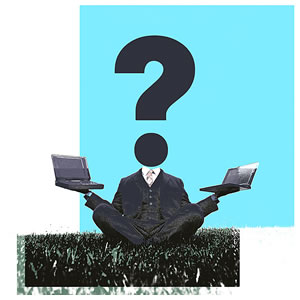
\includegraphics[width=0.4\textwidth]{imgs/preguntas.jpg}
\end{center}
}


\end{document}